The $8$ eyelets for the lace of a sneaker all lie on a rectangle, four equally spaced on each of the longer sides. The rectangle has a width of $50$ mm and a length of $80$ mm. There is one eyelet at each vertex of the rectangle. The lace itself must pass between the vertex eyelets along a width side of the rectangle and then crisscross between successive eyelets until it reaches the two eyelets at the other width side of the rectrangle as shown. After passing through these final eyelets, each of the ends of the lace must extend at least $200$ mm farther to allow a knot to be tied. Find the minimum length of the lace in millimeters.

\begin{center}
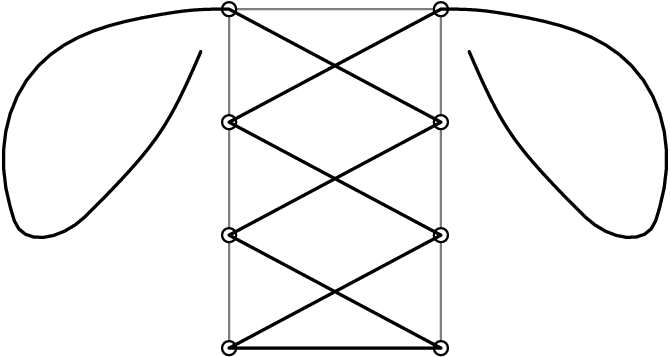
\includegraphics[width = 67.0mm]{img/fig0.png}
\end{center}